\section{Gender Differences}
\label{appendix:genderdifferences}

We summarize (Table~\ref{tab:litreview-table}) work that examines early-life differences between boys and girls. It is generally found that boys are more fragile than girls early in life. While some of these papers consider the family environment, there is a dearth of work studying (1) the effect of low-quality preschool on children\footnote{Although \citet{Kottelenberg-Lehrer_2014_Gender-Effects} study gender gaps, they only consider intact families.} and (2) the interaction of this with family environments. We find that while low-quality programs can deteriorate the parent-child interaction, especially for boys, high-quality programs can enhance it.

\begin{sidewaystable}[H]
\centering
\caption{Literature Review on Early Gender Differences}
\label{tab:litreview-table}
\begin{adjustbox}{width=1.05\textwidth}
\begin{threeparttable}
\begin{tabular}{cccccc} \toprule											
\textbf{Paper}	&	\textbf{Program(s)}	&	\textbf{Main Gender-Difference Finding}	&	\textbf{Outcomes}	&	\textbf{Quality of Childcare Setting?} 	&	\textbf{Quality of Home Setting?} 	\\ \midrule
\citet{lundberg2005sons}	&	Literature survey	&	-females: divorce is likely if all children are girls	&	-fertility and divorce	&	No	&	No	\\ 
	&		&	less likely to live with fathers (US), spends more 	&		&		&		\\ 
	&		&	time with mothers	&		&		&		\\ 
	&		&	-males: increase marital stability, increase 	&		&		&		\\ 
	&		&	likelihood of subsequent child	&		&		&		\\ \\ \midrule
\citet{Anderson_2008_JASA}	&	ABC	&	-modest results for males	&	-child, adolescent, adult (up to age 21 for ABC)	&	No	&	No	\\ 
	&	Perry Preschool Program	&	-females especially affected in academic outcomes	&	-social, educational, employment	&		&		\\ 
	&	Early Training Program (ETP)	&	-accounting for multiple hypotheses	&	-test scores	&		&		\\ 
	&		&		&	reduces effects substantially	&		&		\\ 
	&		&		&	especially for males	&		&		\\ \\ \midrule
\citet{Ou_Reynolds_2010_Mechanisms_CYSR}	&	Chicago Child-Parent Center	&	Differences in treatment effects consequence	&	-educational attainment 	&	No	&	Yes	\\ 
	&	- 1334 youths (682 females, 652 males)	&	of difference in mediators	&	-HS or GED (jointly coded)	&		&		\\ 
	&	- center-based, served 3/4 year olds	&	-male mediators: preschool participation	&		&		&		\\ 
	&	- RCT 	&	-female mediators: family support, abuse/neglect	&		&		&		\\ \\ \midrule
\citet{Bertrand_Pan_2013_AEJAE}	&	ECLS-K (ATUS as complementary)	&	Stark gender differences 	&	-socio-emotional measures	&	No	&	Yes	\\ 
	&	-observational study up to 5th grade	&	- females: better on all socio-emotional measures	&	-grade suspension 	&		&		\\ 
	&		&	(gaps widen when children get older)	&	- tests scores (math and reading)	&		&		\\ 
	&		&	- males: worst at reading but better than math at 	&		&		&		\\ 
	&		&	1st grade	&		&		&		\\ \\ \midrule
\citet{cornwell2013noncognitive}	&	ECLS-K 	&	Gender differences in tests and grades	&	-reading, science, math tests scores 	&	No	&	No	\\ 
	&	-observational study up to 5th grade	&	-males: better in science and math; worst grades	&	-grades	&		&		\\ 
	&		&	overall 	&	-socio-emotional measures	&		&		\\ 
	&		&	females: better reading tests (gap wider than 	&		&		&		\\ 
	&		&	gap with respect to science and math)	&		&		&		\\ 
	&		&	- some but bot all of the gaps disappears when	&		&		&		\\ 
	&		&	accounting for socio-emotional measures 	&		&		&		\\ \\ \midrule
\citet{golsteyn2014gender}	&	Observational study in the Netherlands	&	Gender differences across skills and tests	&	-cognition	&	N/A 	&	No	\\ 
	&	- elementary school children, age 11/12 	&	- males: higher assertiveness and math	&	-socio-emotional measures	&		&		\\ 
	&		&	-females: higher social skills and language	&	-math and language tests	&		&		\\ \\ \midrule
\citet{kottelenberg_Gender}	&	NLSCY	&	-females: better parent-child relationship and 	&	-cognition	&	No	&	Yes	\\ 
	&		&	interactions across diverse measures	&	- socio-emotional outcomes	&		&		\\ 
	&		&	- no precise difference in cognition	&	-parental child relationship and quality of interactions	&		&		\\ 
	&		&		&	-maternal labor supply	&		&		\\ \\ \midrule
\citet{Baker-Milligan_2013_Boy-Girl-Differences}	&	Observational studies in three countries	&	Gender differences in parental investment 	&	-parental investment across different ages	&	No	&	Yes	\\ 
	&	-Canada: NLSCY (ages 1 to 5)	&	-no difference in mother's time at home 	&		&		&		\\ 
	&	-UK: Millennium Cohort Study (ages 1 to 7)	&	-females: more investment in teaching activities	&		&		&		\\ 
	&	-US: ECLS-B (ages 1 to 4)	&	-males: more father's investment at older ages	&		&		&		\\ \\ \midrule
\citet{Magnuson_Kelchen_Duncan_etal_2016_ECRQ}	&	23 programs (meta-analysis)	&	No gender differences, in general	&	-all programs: cognition	&	No	&	No	\\ 
	&	- at least 10 controls	&	- males/females: cognitive benefits	&	-some programs: achievement, behavior,	&		&		\\ 
	&	- from 1960 to 2013	&	- no effect on behavior or mental health	&	adult outcomes	&		&		\\ 
	&	- $<$ 50\%attrition	&		&		&		&		\\ 
	&	- RCTs	&		&		&		&		\\ \\ \midrule
\citet{Schore_2017_IMHJ}	&	Literature survey	&	Sex differences in brain maturation 	&	- brain maturation (right brain development)	&	N/A	&	Yes	\\ 
	&		&	-males: less time spent with mothers, more	&	- daycare behavior	&		&		\\ 
	&		&	sensitive to early infections and endotoxins; 	&	- maternal interaction 	&		&		\\ 
	&		&	respond poorly to daycare settings; amplify stress	&		&		&		\\ 
	&		&	more sensitive to single mother environment	&		&		&		\\ 
	&		&	-females: more rapid brain maturation	&		&		&		\\ \bottomrule
\end{tabular}											
\begin{tablenotes}
\Large
\item Note: This table presents a summary of papers studying early-life gender differences. (1) lists the paper; (2) lists the main program or sample of analysis; (3) lists the main finding with respect to gender differences; (4) the outcomes analyzed; (5) reports if the paper assesses or discusses the quality of the childcare setting; (6) reports if the paper assesses or discusses measures of home quality.
\end{tablenotes}
\end{threeparttable}
\end{adjustbox}
\end{sidewaystable} 

\subsection{Gender Differences in Treatment Effects}
\label{appendix:gdiff-tes}
The following tables report the gender differences between the control means and the treatment effects.

\begin{table}[!htbp]
\centering
\begin{threeparttable}
\caption{Gender Differences of Treatment Effects, IQ}
\begin{scriptsize}
\begin{tabular}{l c c c r c c c r}
\toprule
 \mc{1}{c}{Variable} & \mc{4}{c}{\textbf{Control Mean}} & \mc{4}{c}{\textbf{Treatment Effect}} \\
\cmidrule(lr){2-5} \cmidrule(lr){6-9}
& Male & Female & Difference & $ p $ -value & Male & Female & Difference & $ p $ -value \\
\midrule
IQ, 2 years & 87.265 & 86.000 & 1.265 & 0.180 & 9.528 & 10.700 & -1.172 & 0.180 \\
IQ, 3 years & 88.853 & 86.000 & 2.853 & 0.180 & 13.410 & 13.333 & 0.078 & 0.655 \\
IQ, 3.5 years & 94.206 & 94.743 & -0.537 & 0.655 & 8.756 & 8.049 & 0.708 & 0.655 \\
IQ, 4 years & 90.412 & 91.457 & -1.045 & 0.655 & 12.089 & 6.035 & 6.054 & 0.655 \\
IQ, 4.5 years & 93.118 & 91.529 & 1.588 & 0.180 & 8.508 & 8.162 & 0.346 & 0.655 \\
IQ, 5 years & 94.214 & 95.735 & -1.521 & 0.655 & 7.697 & 4.921 & 2.775 & 0.655 \\
IQ, 6.5 years & 94.333 & 93.467 & 0.867 & 0.180 & 5.803 & 6.127 & -0.324 & 0.180 \\
IQ, 7 years & 95.379 & 93.357 & 2.022 & 0.180 & 4.390 & 6.365 & -1.976 & 0.180 \\
IQ, 8 years & 93.871 & 93.161 & 0.710 & 0.655 & 4.160 & 5.906 & -1.746 & 0.180 \\
IQ, 12 years & 94.485 & 89.250 & 5.235 & 0.180 & 0.686 & 8.688 & -8.003 & 0.180 \\
IQ, 15 years & 93.364 & 88.240 & 5.124 & 0.180 & 4.447 & 6.467 & -2.020 & 0.180 \\
IQ, 21 years & 87.136 & 84.840 & 2.296 & 0.180 & 1.550 & 7.261 & -5.712 & 0.180 \\
IQ Factor, 2-5 years & -0.343 & -0.331 & -0.013 & 0.655 & 0.831 & 0.644 & 0.187 & 0.655 \\
IQ Factor, 6.5-12 years & -0.161 & -0.262 & 0.101 & 0.655 & 0.414 & 0.528 & -0.114 & 0.180 \\
IQ Factor, 15-21 years & -0.003 & -0.319 & 0.316 & 0.180 & 0.252 & 0.615 & -0.363 & 0.180 \\
\bottomrule
\end{tabular}
% This file generated by: abccare-cba/scripts/abccare/genderdifferences/abccare-gdiff-tedifferences-all.do

\end{scriptsize}
\begin{tablenotes}
\scriptsize
Note: This table reproduces the control-group means and estimated treatment effects reported in (1) in Tables~\ref{table:tescombinedmales} and~\ref{table:tescombinedfemales}. The difference columns show the difference between the control mean and treatment effect of males and females. The $p$-value corresponding to each difference is from a sign rank test that compares the empirical distributions over 100 bootstrapped resamples.
\end{tablenotes}
\end{threeparttable}
\end{table}

\begin{table}[!htbp]
\centering
\begin{threeparttable}
\caption{Gender Differences of Treatment Effects, Achievement}
\begin{scriptsize}
\begin{tabular}{l l c c c c r c c c r}
\toprule
\mc{1}{c}{Category} & \mc{1}{c}{Variable} & \mc{1}{c}{Age} & \mc{4}{c}{\textbf{Control Mean}} & \mc{4}{c}{\textbf{Treatment Effect}} \\
\cmidrule(lr){4-7} \cmidrule(lr){8-11}
&   & & Male & Female & Difference & $ p $ -value & Male & Female & Difference & $ p $ -value \\
\midrule
 & Achievement, Total, 5.5 years &  & 93.021 & 92.252 & 0.769 & 0.109 & 5.108 & 12.314 & -7.206 & 0.109 \\
 & Achievement, Total, 6 years &  & 96.794 & 96.310 & 0.483 & 0.285 & 3.091 & 6.269 & -3.178 & 0.109 \\
 &  &  & 94.400 & 93.381 & 1.019 & 0.109 & 1.708 & 3.909 & -2.201 & 0.285 \\
 &  &  & 97.165 & 93.709 & 3.456 & 0.109 & 0.622 & 6.411 & -5.789 & 0.109 \\
 & Achievement, Total, 7.5 years &  & 88.520 & 85.915 & 2.605 & 0.109 & 0.019 & 4.133 & -4.113 & 0.109 \\
 & Achievement, Total, 8 years &  & 93.384 & 91.931 & 1.453 & 0.109 & 2.309 & 6.619 & -4.311 & 0.109 \\
 & Achievement, Total, 8.5 years &  & 88.951 & 88.146 & 0.805 & 0.593 & 3.910 & 8.407 & -4.497 & 0.109 \\
 &  &  & 90.107 & 87.037 & 3.070 & 0.109 & 2.404 & 9.631 & -7.227 & 0.109 \\
 &  &  & 89.727 & 87.552 & 2.175 & 0.109 & 2.231 & 8.275 & -6.044 & 0.109 \\
 & Achievement, Total, 21 years &  & 88.636 & 84.160 & 4.476 & 0.109 & 1.181 & 9.116 & -7.936 & 0.109 \\
 &  &  & -0.449 & -0.276 & -0.173 & 0.109 & 0.594 & 0.822 & -0.228 & 0.109 \\
 &  &  & -0.067 & -0.339 & 0.272 & 0.109 & 0.145 & 0.724 & -0.579 & 0.109 \\
\bottomrule
\end{tabular}
% This file generated by: abccare-cba/scripts/abccare/genderdifferences/abccare-gdiff-tedifferences-all.do

\end{scriptsize}
\begin{tablenotes}
\scriptsize
Note: This table reproduces the control-group means and estimated treatment effects reported in (1) in Tables~\ref{table:tescombinedmales} and~\ref{table:tescombinedfemales}. The difference columns show the difference between the control mean and treatment effect of males and females. The $p$-value corresponding to each difference is from a sign rank test that compares the empirical distributions over 100 bootstrapped resamples.
\end{tablenotes}
\end{threeparttable}
\end{table}

\begin{table}[!htbp]
\centering
\begin{threeparttable}
\caption{Gender Differences of Treatment Effects, Social-emotional}
\begin{scriptsize}
\begin{tabular}{l c c c r c c c r}
\toprule
 \mc{1}{c}{Variable} & \mc{4}{c}{\textbf{Control Mean}} & \mc{4}{c}{\textbf{Treatment Effect}} \\
\cmidrule(lr){2-5} \cmidrule(lr){6-9}
& Male & Female & Difference & $ p $ -value & Male & Female & Difference & $ p $ -value \\
\midrule
IBR, task orientation 2 years & 21.000 & 21.880 & -0.880 & 0.655 & 2.382 & 1.371 & 1.011 & 0.655 \\
IBR, activity level 2 years & 15.643 & 14.654 & 0.989 & 0.180 & -1.786 & 0.383 & -2.169 & 0.180 \\
IBR, cooperation 2 years & 26.750 & 30.444 & -3.694 & 0.180 & 3.752 & 0.556 & 3.197 & 0.180 \\
IBR, task orientation 1.5 years & 20.676 & 21.083 & -0.407 & 0.655 & 1.861 & 2.939 & -1.078 & 0.180 \\
IBR, activity level 1.5 years & 15.235 & 15.222 & 0.013 & 0.180 & -0.917 & -0.045 & -0.872 & 0.180 \\
IBR, cooperation 1.5 years & 24.917 & 28.444 & -3.528 & 0.180 & 1.829 & -0.944 & 2.774 & 0.655 \\
IBR, sociability 1.5 years & 11.147 & 11.057 & 0.090 & 0.180 & -0.710 & 1.074 & -1.784 & 0.180 \\
IBR, task orientation 1 year & 21.143 & 20.694 & 0.448 & 0.180 & 0.896 & 0.940 & -0.044 & 0.180 \\
IBR, activity level 1 year & 13.000 & 13.029 & -0.029 & 0.655 & 0.886 & 1.280 & -0.394 & 0.180 \\
IBR, cooperation 1 year & 26.333 & 26.222 & 0.111 & 0.180 & -2.581 & 4.111 & -6.692 & 0.180 \\
IBR, sociability 1 year & 10.361 & 11.250 & -0.889 & 0.180 & 0.246 & 0.527 & -0.282 & 0.180 \\
IBR, task orientation 6 months & 20.108 & 19.611 & 0.497 & 0.180 & -0.300 & 0.145 & -0.446 & 0.180 \\
IBR, activity level 6 months & 12.514 & 11.111 & 1.402 & 0.180 & -0.097 & 1.278 & -1.375 & 0.180 \\
IBR, cooperation 6 months & 26.154 & 26.444 & -0.291 & 0.655 & 0.016 & 1.156 & -1.140 & 0.655 \\
IBR, sociability 6 months & 10.297 & 10.361 & -0.064 & 0.180 & -0.228 & 0.240 & -0.468 & 0.180 \\
IBR, task orientation 3 months & 11.000 & 11.107 & -0.107 & 0.655 & 0.393 & -0.969 & 1.362 & 0.180 \\
IBR, activity level 3 months & 13.333 & 11.963 & 1.370 & 0.180 & 0.060 & -0.187 & 0.246 & 0.655 \\
IBR, sociability 3 months & 9.348 & 9.500 & -0.152 & 0.655 & -0.312 & -0.372 & 0.060 & 0.655 \\
IBR, task oreination 9 months & 19.542 & 21.333 & -1.792 & 0.180 & 1.070 & 0.654 & 0.416 & 0.180 \\
IBR, activity level 9 months & 11.375 & 12.259 & -0.884 & 0.180 & 0.529 & -1.036 & 1.565 & 0.180 \\
IBR, sociability 9 months & 10.542 & 11.148 & -0.606 & 0.180 & 0.107 & 0.306 & -0.199 & 0.180 \\
IBR, sociability 2 years & 10.353 & 10.882 & -0.529 & 0.180 & -0.145 & 0.232 & -0.377 & 0.180 \\
\bottomrule
\end{tabular}
% This file generated by: abccare-cba/scripts/abccare/genderdifferences/abccare-gdiff-tedifferences-all.do

\end{scriptsize}
\begin{tablenotes}
\scriptsize
Note: This table reproduces the control-group means and estimated treatment effects reported in (1) in Tables~\ref{table:tescombinedmales} and~\ref{table:tescombinedfemales}. The difference columns show the difference between the control mean and treatment effect of males and females. The $p$-value corresponding to each difference is from a sign rank test that compares the empirical distributions over 100 bootstrapped resamples.
\end{tablenotes}
\end{threeparttable}
\end{table}


\begin{table}[!htbp]
\centering
\begin{threeparttable}
\caption{Gender Differences of Treatment Effects, Parenting}
\begin{scriptsize}
\begin{tabular}{l c c c r c c c r}
\toprule
 \mc{1}{c}{Variable} & \mc{4}{c}{\textbf{Control Mean}} & \mc{4}{c}{\textbf{Treatment Effect}} \\
\cmidrule(lr){2-5} \cmidrule(lr){6-9}
& Male & Female & Difference & $ p $ -value & Male & Female & Difference & $ p $ -value \\
\midrule
HOME, 6 months & 27.946 & 26.417 & 1.529 & $ < $ 0.001 & 0.372 & 1.581 & -1.209 & $ < $ 0.001 \\
HOME, 1.5 years & 30.529 & 27.278 & 3.252 & $ < $ 0.001 & -0.500 & 2.668 & -3.168 & $ < $ 0.001 \\
HOME, 2.5 years & 29.500 & 29.417 & 0.083 & 0.465 & 0.141 & 0.762 & -0.621 & 0.070 \\
HOME, 3.5 years & 54.939 & 54.114 & 0.825 & 0.051 & 1.404 & 2.858 & -1.453 & 0.018 \\
HOME, 4.5 years & 58.794 & 56.061 & 2.734 & $ < $ 0.001 & 1.146 & 2.736 & -1.590 & 0.001 \\
HOME, 8 years & 65.333 & 66.296 & -0.963 & 0.023 & 1.548 & 0.659 & 0.888 & 0.048 \\
HOME Factor, 6 months - 8 years & -0.125 & -0.181 & 0.056 & 0.066 & 0.266 & 0.262 & 0.005 & 0.963 \\
\bottomrule
\end{tabular}
% This file generated by: abccare-cba/scripts/abccare/genderdifferences/abccare-gdiff-tedifferences-all.do

\end{scriptsize}
\begin{tablenotes}
\scriptsize
Note: This table reproduces the control-group means and estimated treatment effects reported in (1) in Tables~\ref{table:tescombinedmales} and~\ref{table:tescombinedfemales}. The difference columns show the difference between the control mean and treatment effect of males and females. The $p$-value corresponding to each difference is from a sign rank test that compares the empirical distributions over 100 bootstrapped resamples.
\end{tablenotes}
\end{threeparttable}
\end{table}


\begin{table}[!htbp]
\centering
\begin{threeparttable}
\caption{Gender Differences of Treatment Effects, Parental Income}
\begin{scriptsize}
\begin{tabular}{l c c c r c c c r}
\toprule
 \mc{1}{c}{Variable} & \mc{4}{c}{\textbf{Control Mean}} & \mc{4}{c}{\textbf{Treatment Effect}} \\
\cmidrule(lr){2-5} \cmidrule(lr){6-9}
& Male & Female & Difference & $ p $ -value & Male & Female & Difference & $ p $ -value \\
\midrule
Parental income, 1.5 years & 15704.771 & 11435.556 & 4,269.216 & 0.180 & 329.530 & 4,515.554 & -4186.023 & 0.655 \\
Parental income, 2.5 years & 14465.235 & 13557.772 & 907.463 & 0.180 & 673.032 & 221.637 & 451.395 & 0.180 \\
Parental income, 3.5 years & 13504.955 & 11464.967 & 2,039.988 & 0.180 & 1,035.575 & 2,755.646 & -1720.072 & 0.655 \\
Parental income, 4.5 years & 19001.697 & 15620.230 & 3,381.467 & 0.180 & 820.780 & 4,038.564 & -3217.785 & 0.180 \\
Parental income, 8 years & 19915.480 & 21671.717 & -1756.236 & 0.655 & 11786.443 & 2,180.545 & 9,605.898 & 0.180 \\
Parental income, 12 years & 23868.104 & 20917.408 & 2,950.695 & 0.180 & 7,085.101 & 13632.505 & -6547.404 & 0.180 \\
Parental income, 15 years & 22985.377 & 13772.383 & 9,212.994 & 0.180 & 8,487.858 & 8,564.723 & -76.864 & 0.180 \\
Parental income, 21 years & 21584.943 & 20803.541 & 781.402 & 0.180 & 12732.085 & 5,707.595 & 7,024.490 & 0.180 \\
Parental income Factor, 1.5-21 years & 0.020 & 0.002 & 0.018 & 0.180 & -0.128 & 0.110 & -0.237 & 0.655 \\
Mother works, 1.5 years & 0.824 & 0.722 & 0.101 & 0.180 & 0.056 & 0.168 & -0.113 & 0.180 \\
Mother works, 2.5 years & 0.719 & 0.750 & -0.031 & 0.655 & 0.150 & 0.087 & 0.063 & 0.180 \\
Mother works, 3.5 years & 0.765 & 0.750 & 0.015 & 0.180 & 0.134 & 0.118 & 0.016 & 0.655 \\
Mother works, 4.5 years & 0.758 & 0.794 & -0.037 & 0.655 & 0.111 & 0.067 & 0.044 & 0.655 \\
Mother works, 21 years & 0.762 & 0.750 & 0.012 & 0.180 & -0.058 & -0.018 & -0.041 & 0.180 \\
Mother works Factor, 1.5-21 years & -0.452 & 0.091 & -0.543 & 0.655 & 0.528 & -0.008 & 0.536 & 0.655 \\
\bottomrule
\end{tabular}
% This file generated by: abccare-cba/scripts/abccare/genderdifferences/abccare-gdiff-tedifferences-all.do

\end{scriptsize}
\begin{tablenotes}
\scriptsize
Note: This table reproduces the control-group means and estimated treatment effects reported in (1) in Tables~\ref{table:tescombinedmales} and~\ref{table:tescombinedfemales}. The difference columns show the difference between the control mean and treatment effect of males and females. The $p$-value corresponding to each difference is from a sign rank test that compares the empirical distributions over 100 bootstrapped resamples.
\end{tablenotes}
\end{threeparttable}
\end{table}


\begin{table}[!htbp]
\centering
\begin{threeparttable}
\caption{Gender Differences of Treatment Effects, Education}
\begin{scriptsize}
\begin{tabular}{l c c c r c c c r}
\toprule
 \mc{1}{c}{Variable} & \mc{4}{c}{\textbf{Control Mean}} & \mc{4}{c}{\textbf{Treatment Effect}} \\
\cmidrule(lr){2-5} \cmidrule(lr){6-9}
& Male & Female & Difference & $ p $ -value & Male & Female & Difference & $ p $ -value \\
\midrule
Graduated high school, 30 years & 0.600 & 0.529 & 0.071 & 0.013 & 0.073 & 0.253 & -0.180 & $ < $ 0.001 \\
Attended vocational program, 30 years & 0.633 & 0.735 & -0.102 & $ < $ 0.001 & -0.099 & -0.057 & -0.042 & 0.290 \\
Graduated from 4-year college, 30 years & 0.120 & 0.088 & 0.032 & 0.022 & 0.170 & 0.134 & 0.036 & 0.001 \\
Years of education, 30 years & 12.867 & 11.794 & 1.073 & $ < $ 0.001 & 0.525 & 2.143 & -1.618 & $ < $ 0.001 \\
Ever in special education, 18 years & 0.750 & 0.576 & 0.174 & $ < $ 0.001 & -0.035 & 0.022 & -0.057 & 0.001 \\
Number of years in special education, 18 years & 3.625 & 3.061 & 0.564 & $ < $ 0.001 & -0.544 & -0.622 & 0.079 & 0.453 \\
Ever retained, 18 years & 0.500 & 0.576 & -0.076 & 0.001 & -0.095 & -0.256 & 0.161 & $ < $ 0.001 \\
Number of years retained, 18 years & 0.531 & 0.667 & -0.135 & $ < $ 0.001 & -0.070 & -0.233 & 0.163 & $ < $ 0.001 \\
Education Factor & 0.125 & 0.238 & -0.113 & $ < $ 0.001 & -0.307 & -0.577 & 0.270 & $ < $ 0.001 \\
\bottomrule
\end{tabular}
% This file generated by: abccare-cba/scripts/abccare/genderdifferences/abccare-gdiff-tedifferences-all.do

\end{scriptsize}
\begin{tablenotes}
\scriptsize
Note: This table reproduces the control-group means and estimated treatment effects reported in (1) in Tables~\ref{table:tescombinedmales} and~\ref{table:tescombinedfemales}. The difference columns show the difference between the control mean and treatment effect of males and females. The $p$-value corresponding to each difference is from a sign rank test that compares the empirical distributions over 100 bootstrapped resamples.
\end{tablenotes}
\end{threeparttable}
\end{table}


\begin{table}[!htbp]
\centering
\begin{threeparttable}
\caption{Gender Differences of Treatment Effects, Employment}
\begin{scriptsize}
\begin{tabular}{l c c c r c c c r}
\toprule
 \mc{1}{c}{Variable} & \mc{4}{c}{\textbf{Control Mean}} & \mc{4}{c}{\textbf{Treatment Effect}} \\
\cmidrule(lr){2-5} \cmidrule(lr){6-9}
& Male & Female & Difference & $ p $ -value & Male & Female & Difference & $ p $ -value \\
\midrule
Employed, 30 years & 0.700 & 0.706 & -0.006 & 0.373 & 0.119 & 0.131 & -0.012 & 0.903 \\
Labor income, 21 years & 17711.383 & 11030.102 & 6,681.281 & $ < $ 0.001 & -1671.961 & 1,741.474 & -3413.435 & $ < $ 0.001 \\
Labor income, 30 years & 30078.938 & 23267.205 & 6,811.732 & $ < $ 0.001 & 19809.742 & 2,547.503 & 17262.240 & $ < $ 0.001 \\
Employment Factor & -0.085 & -0.106 & 0.020 & 0.694 & 0.281 & 0.107 & 0.174 & $ < $ 0.001 \\
\bottomrule
\end{tabular}
% This file generated by: abccare-cba/scripts/abccare/genderdifferences/abccare-gdiff-tedifferences-all.do

\end{scriptsize}
\begin{tablenotes}
\scriptsize
Note: This table reproduces the control-group means and estimated treatment effects reported in (1) in Tables~\ref{table:tescombinedmales} and~\ref{table:tescombinedfemales}. The difference columns show the difference between the control mean and treatment effect of males and females. The $p$-value corresponding to each difference is from a sign rank test that compares the empirical distributions over 100 bootstrapped resamples.
\end{tablenotes}
\end{threeparttable}
\end{table}


\begin{table}[!htbp]
\centering
\begin{threeparttable}
\caption{Gender Differences of Treatment Effects, Crime}
\begin{scriptsize}
\begin{tabular}{l l c c c c r c c c r}
\toprule
\mc{1}{c}{Category} & \mc{1}{c}{Variable} & \mc{1}{c}{Age} & \mc{4}{c}{\textbf{Control Mean}} & \mc{4}{c}{\textbf{Treatment Effect}} \\
\cmidrule(lr){4-7} \cmidrule(lr){8-11}
&   & & Male & Female & Difference & $ p $ -value & Male & Female & Difference & $ p $ -value \\
\midrule
Crime & Total Felony Arrests & Mid-30s & -1.370 & -0.419 & -0.951 & 0.109 & -0.196 & 0.328 & -0.524 & 0.285 \\
 & Total Misdemeanor Arrests & Mid-30s & -1.296 & -1.161 & -0.135 & 1.000 & 0.501 & 0.973 & -0.472 & 0.285 \\
 &  &  & -0.216 & -0.027 & -0.189 & 0.109 & -0.348 & 0.024 & -0.372 & 0.109 \\
 &  &  & -0.157 & 0.178 & -0.335 & 0.109 & -0.169 & 0.155 & -0.324 & 0.109 \\
\bottomrule
\end{tabular}
% This file generated by: abccare-cba/scripts/abccare/genderdifferences/abccare-gdiff-tedifferences-all.do

\end{scriptsize}
\begin{tablenotes}
\scriptsize
Note: This table reproduces the control-group means and estimated treatment effects reported in (1) in Tables~\ref{table:tescombinedmales} and~\ref{table:tescombinedfemales}. The difference columns show the difference between the control mean and treatment effect of males and females. The $p$-value corresponding to each difference is from a sign rank test that compares the empirical distributions over 100 bootstrapped resamples.
\end{tablenotes}
\end{threeparttable}
\end{table}


\begin{table}[!htbp]
\centering
\begin{threeparttable}
\caption{Gender Differences of Treatment Effects, Risky Behavior}
\begin{scriptsize}
\begin{tabular}{l l c c c c r c c c r}
\toprule
\mc{1}{c}{Category} & \mc{1}{c}{Variable} & \mc{1}{c}{Age} & \mc{4}{c}{\textbf{Control Mean}} & \mc{4}{c}{\textbf{Treatment Effect}} \\
\cmidrule(lr){4-7} \cmidrule(lr){8-11}
&   & & Male & Female & Difference & $ p $ -value & Male & Female & Difference & $ p $ -value \\
\midrule
 &  &  & -2.810 & -3.544 & 0.734 & 1.000 & -0.826 & 0.765 & -1.591 & 1.000 \\
 &  &  & -5.293 & -3.662 & -1.631 & 0.109 & -0.805 & 0.742 & -1.547 & 1.000 \\
 &  &  & -0.862 & -1.088 & 0.226 & 0.593 & -0.500 & 0.358 & -0.858 & 1.000 \\
Health & Self-reported drug user & Mid-30s & -0.500 & -0.259 & -0.241 & 0.109 & 0.333 & 0.033 & 0.301 & 0.109 \\
 &  &  & 0.059 & 0.145 & -0.086 & 0.109 & -0.337 & -0.006 & -0.331 & 1.000 \\
\bottomrule
\end{tabular}
% This file generated by: abccare-cba/scripts/abccare/genderdifferences/abccare-gdiff-tedifferences-all.do

\end{scriptsize}
\begin{tablenotes}
\scriptsize
Note: This table reproduces the control-group means and estimated treatment effects reported in (1) in Tables~\ref{table:tescombinedmales} and~\ref{table:tescombinedfemales}. The difference columns show the difference between the control mean and treatment effect of males and females. The $p$-value corresponding to each difference is from a sign rank test that compares the empirical distributions over 100 bootstrapped resamples.
\end{tablenotes}
\end{threeparttable}
\end{table}

\begin{table}[!htbp]
\centering
\begin{threeparttable}
\caption{Gender Differences of Treatment Effects, Health}
\begin{scriptsize}
\begin{tabular}{l c c c r c c c r}
\toprule
 \mc{1}{c}{Variable} & \mc{4}{c}{\textbf{Control Mean}} & \mc{4}{c}{\textbf{Treatment Effect}} \\
\cmidrule(lr){2-5} \cmidrule(lr){6-9}
& Male & Female & Difference & $ p $ -value & Male & Female & Difference & $ p $ -value \\
\midrule
Self-reported health, 30 years & 2.000 & 1.853 & 0.147 & $ < $ 0.001 & -0.004 & -0.184 & 0.180 & $ < $ 0.001 \\
Self-reported health, mid 30s & 2.286 & 2.444 & -0.159 & 0.022 & 0.196 & 0.006 & 0.190 & 0.009 \\
Self-reported health Factor & -0.037 & 0.025 & -0.062 & 0.090 & -0.035 & 0.045 & -0.080 & 0.020 \\
Systolic blood pressure, mid 30s & 138.071 & 133.963 & 4.108 & 0.062 & -9.791 & -2.899 & -6.892 & 0.001 \\
Diastolic blood pressure, mid 30s & 89.214 & 87.556 & 1.659 & 0.415 & -10.854 & -0.002 & -10.853 & $ < $ 0.001 \\
Prehypertensive, mid 30s & 0.857 & 0.926 & -0.069 & $ < $ 0.001 & -0.137 & -0.189 & 0.052 & 0.120 \\
Hypertensive, mid 30s & 0.571 & 0.407 & 0.164 & $ < $ 0.001 & -0.291 & 0.172 & -0.464 & $ < $ 0.001 \\
Hypertension Factor & 0.280 & 0.113 & 0.167 & 0.038 & -0.599 & -0.033 & -0.566 & $ < $ 0.001 \\
HDL Cholesterol, mid 30s & 43.647 & 54.333 & -10.686 & $ < $ 0.001 & 7.753 & 2.884 & 4.869 & 0.001 \\
Dyslipidemia, mid 30s & 0.294 & 0.037 & 0.257 & $ < $ 0.001 & -0.094 & 0.051 & -0.145 & $ < $ 0.001 \\
Cholesterol Factor & 0.431 & -0.176 & 0.607 & $ < $ 0.001 & -0.333 & -0.024 & -0.309 & $ < $ 0.001 \\
Hemoglobin, mid 30s & 5.618 & 5.863 & -0.245 & $ < $ 0.001 & 0.322 & -0.277 & 0.599 & $ < $ 0.001 \\
Prediabetic, mid 30s & 0.529 & 0.296 & 0.233 & $ < $ 0.001 & -0.129 & 0.088 & -0.217 & $ < $ 0.001 \\
Diabetic, mid 30s & 0.000 & 0.074 & -0.074 & $ < $ 0.001 & 0.080 & -0.071 & 0.151 & $ < $ 0.001 \\
Diabetes Factor & -0.138 & 0.083 & -0.222 & $ < $ 0.001 & 0.283 & -0.249 & 0.532 & $ < $ 0.001 \\
BMI, mid 30s & 31.164 & 34.224 & -3.060 & $ < $ 0.001 & -0.125 & 3.545 & -3.669 & $ < $ 0.001 \\
Obese, mid 30s & 0.538 & 0.741 & -0.202 & $ < $ 0.001 & -0.000 & -0.011 & 0.011 & 0.437 \\
Severely obese, mid 30s & 0.308 & 0.370 & -0.063 & 0.014 & -0.160 & -0.045 & -0.115 & 0.005 \\
Waist-hip ratio, mid 30s & 0.937 & 0.925 & 0.012 & 0.006 & 0.005 & -0.022 & 0.027 & $ < $ 0.001 \\
Obese waist-hip ratio, mid 30s & 0.692 & 0.769 & -0.077 & 0.015 & 0.003 & -0.159 & 0.162 & $ < $ 0.001 \\
Framingham score, mid 30s & 5.951 & 1.323 & 4.628 & $ < $ 0.001 & -0.766 & -0.259 & -0.507 & 0.014 \\
Body mass Factor & -0.116 & 0.030 & -0.146 & 0.023 & -0.040 & 0.088 & -0.128 & 0.196 \\
\bottomrule
\end{tabular}
% This file generated by: abccare-cba/scripts/abccare/genderdifferences/abccare-gdiff-tedifferences-all.do

\end{scriptsize}
\begin{tablenotes}
\scriptsize
Note: This table reproduces the control-group means and estimated treatment effects reported in (1) in Tables~\ref{table:tescombinedmales} and~\ref{table:tescombinedfemales}. The difference columns show the difference between the control mean and treatment effect of males and females. The $p$-value corresponding to each difference is from a sign rank test that compares the empirical distributions over 100 bootstrapped resamples.
\end{tablenotes}
\end{threeparttable}
\end{table}

\begin{table}[!htbp]
\centering
\begin{threeparttable}
\caption{Gender Differences of Treatment Effects, Mental Health}
\begin{scriptsize}
\begin{tabular}{l c c c r c c c r}
\toprule
 \mc{1}{c}{Variable} & \mc{4}{c}{\textbf{Control Mean}} & \mc{4}{c}{\textbf{Treatment Effect}} \\
\cmidrule(lr){2-5} \cmidrule(lr){6-9}
& Male & Female & Difference & $ p $ -value & Male & Female & Difference & $ p $ -value \\
\midrule
Somitization, 21 years & 54.364 & 53.242 & 1.121 & 0.006 & -2.804 & -2.671 & -0.134 & 0.722 * \\
Somitaization, 30 years & 49.214 & 48.185 & 1.029 & 0.213 * & -3.066 & 0.724 & -3.790 & 0.021 * \\
Depression, 21 years & 54.419 & 58.848 & -4.429 & 0.003 & -2.515 & -5.649 & 3.134 & 0.013 \\
Depression, 30 years & 50.857 & 52.222 & -1.365 & 0.213 * & -1.042 & -2.466 & 1.424 & 0.657 * \\
Anxiety, 21 years & 55.000 & 56.545 & -1.545 & 0.424 * & 0.400 & -6.163 & 6.563 & 0.003 \\
Anxiety, 30 years & 47.143 & 49.000 & -1.857 & 0.182 * & -1.847 & -4.564 & 2.717 & 0.182 * \\
Hostility, 21 years & 57.812 & 64.364 & -6.551 & 0.003 & -1.471 & -4.721 & 3.251 & 0.004 \\
Hostility, 30 years & 47.000 & 49.741 & -2.741 & 0.110 * & -1.556 & 0.512 & -2.068 & 0.248 * \\
Global Severity Index, 21 years & 57.867 & 62.455 & -4.588 & 0.003 & 0.246 & -6.436 & 6.682 & 0.003 \\
Global Severity Index, 30 years & 43.786 & 46.815 & -3.029 & 0.033 * & -1.675 & -2.365 & 0.690 & 0.859 * \\
Mental health Factor & -0.128 & 0.479 & -0.607 & 0.003 & -0.172 & -0.622 & 0.450 & 0.010 \\
\bottomrule
\end{tabular}
% This file generated by: abccare-cba/scripts/abccare/genderdifferences/abccare-gdiff-tedifferences-all.do

\end{scriptsize}
\begin{tablenotes}
\scriptsize
Note: This table reproduces the control-group means and estimated treatment effects reported in (1) in Tables~\ref{table:tescombinedmales} and~\ref{table:tescombinedfemales}. The difference columns show the difference between the control mean and treatment effect of males and females. The $p$-value corresponding to each difference is from a sign rank test that compares the empirical distributions over 100 bootstrapped resamples.
\end{tablenotes}
\end{threeparttable}
\end{table}

\subsection{Proportion of Outcomes Males $>$ Females}
\label{appendix:propmales-females}

Tables~\ref{tab:proportion-table-home} and~\ref{tab:proportion-table-alt} show the analogue of Table~\ref{tab:proportion-table} but comparing to subjects in the the control group that stays at home and attend alternative preschool, respectively. Table~\ref{fig:proportion-fhome} partitions the data by whether the father is present.


\begin{table}[H]
\centering
\caption{Summary of Proportion of Outcomes Males $>$ Females, Stay at Home}
\label{tab:proportion-table-home}
\begin{threeparttable}
\begin{tabular}{l c c c c}
\toprule
Category & \# Outcomes & \mc{2}{c}{Proportion} & Difference \\
\cmidrule(lr){3-4} \cmidrule(lr){5-5}
            &                       & Control & Treatment & Treatment $- $ Control \\
\midrule
IQ & 15 & \textbf{1.000} & 0.533 & \textbf{-0.467} \\
Achievement & 12 & \textbf{1.000} & \textbf{0.000} & \textbf{-1.000} \\
Social-Emotional & 22 & 0.591 & \textbf{0.364} & \textbf{-0.227} \\
Parenting & 7 & \textbf{1.000} & 0.286 & \textbf{-0.714} \\
Parental Labor Income & 15 & \textbf{0.800} & 0.733 & \textbf{-0.067} \\
Education & 9 & \textbf{0.667} & \textbf{0.111} & \textbf{-0.556} \\
Employment & 4 & \textbf{1.000} & \textbf{0.750} & \textbf{-0.250} \\
Crime & 4 & 0.500 & \textbf{0.000} & \textbf{-0.500} \\
Risky Behavior & 5 & \textbf{0.200} & \textbf{0.200} & \textbf{0.000} \\
Health & 22 & 0.545 & 0.545 & 0.000 \\
Mental Health & 11 & \textbf{1.000} & 0.545 & \textbf{-0.455} \\
\midrule
All & 126 & \textbf{0.754} & 0.413 & \textbf{-0.341} \\
\bottomrule
\end{tabular}
% This file generated by: abccare-cba/scripts/abccare/genderdifferences/abccare-gdiff-gaps-ranksign.do

\begin{tablenotes}
\footnotesize
\item Note: This table summarizes comparison of gender gaps across outcome categories by different groups. A bold proportion for the treatment or control group indicates that the proportion is statistically different than 50\%. A bold difference between treatment and control indicates that the rank sign test over 100 bootstraps yields a $p$-value less than or equal to 0.10. 
\end{tablenotes}
\end{threeparttable}
\end{table}

\begin{table}[H]
\centering
\caption{Summary of Proportion of Outcomes Males $>$ Females, Alternative Preschool}
\label{tab:proportion-table-alt}
\begin{threeparttable}
\begin{tabular}{l c c c c}
\toprule
Category & \# Outcomes & \mc{2}{c}{Proportion} & Difference \\
\cmidrule(lr){3-4} \cmidrule(lr){5-5}
            &                       & Control & Treatment & Treatment $- $ Control \\
\midrule
IQ & 15 & 0.267 & 0.533 & \textbf{0.267} \\
Achievement & 12 & 0.250 & \textbf{0.000} & \textbf{-0.250} \\
Social-emotional & 22 & \textbf{0.318} & \textbf{0.364} & \textbf{0.045} \\
Parenting & 7 & 0.429 & 0.286 & -0.143 \\
Parental Income & 15 & 0.467 & 0.733 & \textbf{0.267} \\
Education & 9 & 0.444 & \textbf{0.111} & \textbf{-0.333} \\
Employment & 4 & 0.500 & \textbf{0.750} & \textbf{0.250} \\
Crime & 4 & \textbf{0.000} & \textbf{0.000} & \textbf{0.000} \\
Risky Behavior & 5 & 0.600 & \textbf{0.200} & \textbf{-0.400} \\
Health & 22 & 0.500 & 0.545 & \textbf{0.045} \\
Mental Health & 11 & 0.545 & 0.545 & \textbf{0.000} \\
\midrule
All & 126 & 0.397 & 0.413 & \textbf{0.016} \\
\bottomrule
\end{tabular}
% This file generated by: abccare-cba/scripts/abccare/genderdifferences/abccare-gdiff-gaps-ranksign.do

\begin{tablenotes}
\footnotesize
\item Note: This table summarizes comparison of gender gaps across outcome categories by different groups. A bold proportion for the treatment or control group indicates that the proportion is statistically different than 50\%. A bold difference between treatment and control indicates that the rank sign test over 100 bootstraps yields a $p$-value less than or equal to 0.10. 
\end{tablenotes}
\end{threeparttable}
\end{table}

\begin{figure}[!htbp]
\centering
\caption{Proportion of Outcomes Males $>$ Females, by Outcome Category, Partitioning by Whether or Not the Father is Present}
\label{fig:proportion-fhome}
\begin{subfigure}[h]{0.7\textwidth}
	\centering
	\caption{Control Group}
	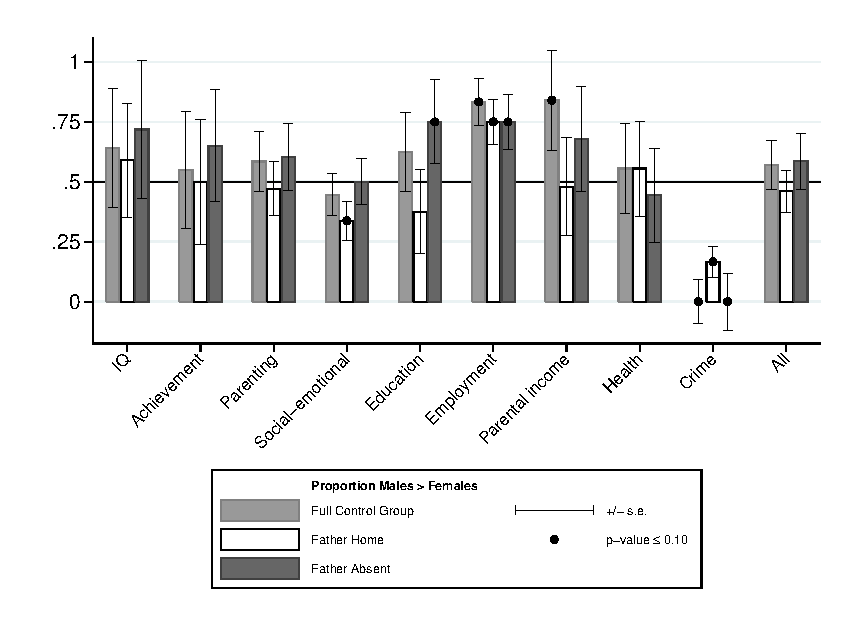
\includegraphics[width=\textwidth]{output/gendergaps-control-moderated-fhome}
	\end{subfigure}
	
\begin{subfigure}[h]{0.7\textwidth}
	\centering
	\caption{Treatment Group}
	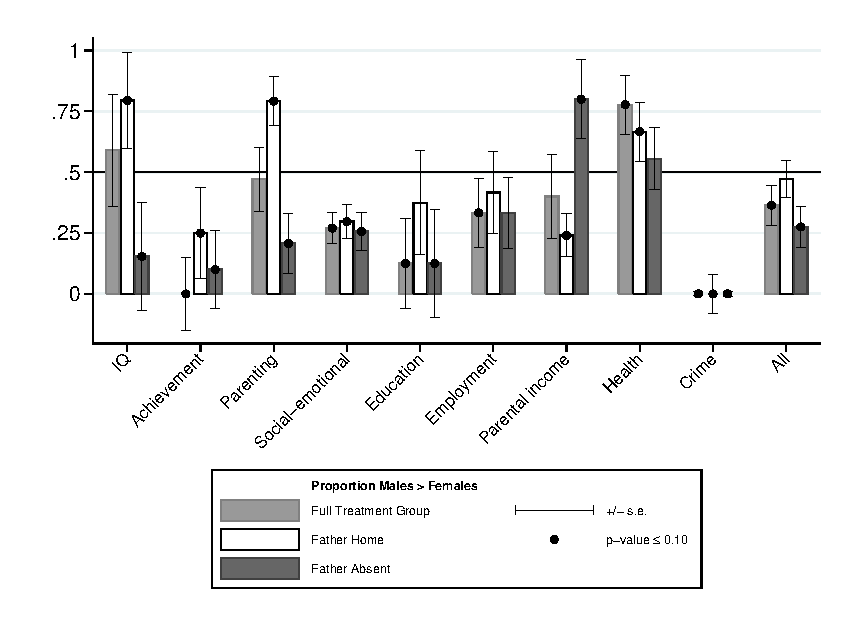
\includegraphics[width=\textwidth]{output/gendergaps-treatment-moderated-fhome}
	\end{subfigure}
\footnotesize \justify
Note: These plots show the proportion of outcomes, by outcome category, for which the males' mean is larger than the females' mean. The standard errors and the $p$-values are computed using 100 bootstraps. The $p$-values are one-sided and test the null hypothesis that the proportion of outcomes is greater than $\frac{1}{2}$ The crime outcomes are all coded so that a higher value indicates more criminal activity. All other outcome categories have higher values corresponding to socially desirable outcomes.
\end{figure}